%%
%% This is file `sample-manuscript.tex',
%% generated with the docstrip utility.
%%
%% The original source files were:
%%
%% samples.dtx  (with options: `manuscript')
%% 
%% IMPORTANT NOTICE:
%% 
%% For the copyright see the source file.
%% 
%% Any modified versions of this file must be renamed
%% with new filenames distinct from sample-manuscript.tex.
%% 
%% For distribution of the original source see the terms
%% for copying and modification in the file samples.dtx.
%% 
%% This generated file may be distributed as long as the
%% original source files, as listed above, are part of the
%% same distribution. (The sources need not necessarily be
%% in the same archive or directory.)
%%
%% Commands for TeXCount
%TC:macro \cite [option:text,text]
%TC:macro \citep [option:text,text]
%TC:macro \citet [option:text,text]
%TC:envir table 0 1
%TC:envir table* 0 1
%TC:envir tabular [ignore] word
%TC:envir displaymath 0 word
%TC:envir math 0 word
%TC:envir comment 0 0
%%
%%
%% The first command in your LaTeX source must be the \documentclass command. This is the generic manuscript mode required for submission and peer review.
\documentclass[manuscript,screen,review]{acmart}
%% To ensure 100% compatibility, please check the white list of
%% approved LaTeX packages to be used with the Master Article Template at
%% https://www.acm.org/publications/taps/whitelist-of-latex-packages 
%% before creating your document. The white list page provides 
%% information on how to submit additional LaTeX packages for 
%% review and adoption.
%% Fonts used in the template cannot be substituted; margin 
%% adjustments are not allowed.
\usepackage{graphicx}
%%
%% \BibTeX command to typeset BibTeX logo in the docs
\AtBeginDocument{%
  \providecommand\BibTeX{{%
    \normalfont B\kern-0.5em{\scshape i\kern-0.25em b}\kern-0.8em\TeX}}}

%% Rights management information.  This information is sent to you
%% when you complete the rights form.  These commands have SAMPLE
%% values in them; it is your responsibility as an author to replace
%% the commands and values with those provided to you when you
%% complete the rights form.
\setcopyright{acmcopyright}
\copyrightyear{2024}
\acmYear{2024}
\acmDOI{XXXXXXX.XXXXXXX}

%% These commands are for a PROCEEDINGS abstract or paper.
% \acmConference[Conference acronym 'XX]{Make sure to enter the correct
%   conference title from your rights confirmation emai}{June 03--05,
%   2018}{Woodstock, NY}
%
%  Uncomment \acmBooktitle if th title of the proceedings is different
%  from ``Proceedings of ...''!
%
%\acmBooktitle{Woodstock '18: ACM Symposium on Neural Gaze Detection,
%  June 03--05, 2018, Woodstock, NY} 

%% These commands are for a JOURNAL article.
\acmJournal{JACM}
\acmVolume{37}
\acmNumber{5}
\acmArticle{111}
\acmMonth{4}

\acmPrice{15.00}
\acmISBN{978-1-4503-XXXX-X/24/04}


%%
%% Submission ID.
%% Use this when submitting an article to a sponsored event. You'll
%% receive a unique submission ID from the organizers
%% of the event, and this ID should be used as the parameter to this command.
%%\acmSubmissionID{123-A56-BU3}

%%
%% For managing citations, it is recommended to use bibliography
%% files in BibTeX format.
%%
%% You can then either use BibTeX with the ACM-Reference-Format style,
%% or BibLaTeX with the acmnumeric or acmauthoryear sytles, that include
%% support for advanced citation of software artefact from the
%% biblatex-software package, also separately available on CTAN.
%%
%% Look at the sample-*-biblatex.tex files for templates showcasing
%% the biblatex styles.
%%

%%
%% The majority of ACM publications use numbered citations and
%% references.  The command \citestyle{authoryear} switches to the
%% "author year" style.
%%
%% If you are preparing content for an event
%% sponsored by ACM SIGGRAPH, you must use the "author year" style of
%% citations and references.
%% Uncommenting
%% the next command will enable that style.
%%\citestyle{acmauthoryear}
\begin{abstract}
  Horror as a genre of entertainment exists in several forms; film, books, comics, video games, and recently as virtual reality video games. We present findings from an experiment about how users heart rate while completing a task before, within, and after playing a virtual reality horror video game changes. Between each of those tasks participant's heart rates were allowed to return to a resting level. Our results show that there was no statistically significant impact on heart rate before and after in participants who did not have an elevated heart rate while playing the game, however, when participants did have an elevated heart rate while playing the game they also had a statistically significant increase in heart rate in the task before and after. These findings shed light on how users may be influenced to feel emotions in both horror and virtual reality even after no longer directly exposed to the direct stimuli.
\end{abstract}

%%
%% end of the preamble, start of the body of the document source.
\begin{document}

%%
%% The "title" command has an optional parameter,
%% allowing the author to define a "short title" to be used in page headers.
\title{Assessing the Impact of Virtual Reality Horror Experiences on Sensitivity to Fear 
Stimuli}

%%
%% The "author" command and its associated commands are used to define
%% the authors and their affiliations.
%% Of note is the shared affiliation of the first two authors, and the
%% "authornote" and "authornotemark" commands
%% used to denote shared contribution to the research.
\author{Joseph Almahmid}
\authornote{Both authors contributed equally to this research.}
\email{zoroko@colostate.edu}
\author{Drew Schmuck}
\email{dschmuck@colostate}
\affiliation{%
  \institution{Colorado State University}
  \city{Fort Collins}
  \state{Colorado}
  \country{USA}
  \postcode{80521}
}

%%
%% By default, the full list of authors will be used in the page
%% headers. Often, this list is too long, and will overlap
%% other information printed in the page headers. This command allows
%% the author to define a more concise list
%% of authors' names for this purpose.
\renewcommand{\shortauthors}{Almahmid and Schmuck}

%%
%% The code below is generated by the tool at http://dl.acm.org/ccs.cfm.
%% Please copy and paste the code instead of the example below.
%%
\begin{CCSXML}
<ccs2012>
   <concept>
       <concept_id>10011007.10011074.10011075.10011077</concept_id>
       <concept_desc>Software and its engineering~Software design engineering</concept_desc>
       <concept_significance>300</concept_significance>
       </concept>
   <concept>
       <concept_id>10002944.10011123.10011131</concept_id>
       <concept_desc>General and reference~Experimentation</concept_desc>
       <concept_significance>500</concept_significance>
       </concept>
   <concept>
       <concept_id>10003120.10003121.10003125.10010591</concept_id>
       <concept_desc>Human-centered computing~Displays and imagers</concept_desc>
       <concept_significance>300</concept_significance>
       </concept>
 </ccs2012>
\end{CCSXML}

\ccsdesc[300]{Software and its engineering~Software design engineering}
\ccsdesc[500]{General and reference~Experimentation}
\ccsdesc[300]{Human-centered computing~Displays and imagers}

%%
%% Keywords. The author(s) should pick words that accurately describe
%% the work being presented. Separate the keywords with commas.
\keywords{virtual reality, physiological information measurement, fear elicitation}

%%
%% This command processes the author and affiliation and title
%% information and builds the first part of the formatted document.
\maketitle

\section{Introduction}

Ever since the commercial release of the Occulus DK1 virtual reality(VR) headset in 2013, the technology has become more and more prominent as a commercial product. What was once something that mostly used by researchers or seen in arcades became a product that users could buy for a reasonable price and use in their own homes. This trend can be further seen by entry level headsets, such as the Meta Quest 2, being sold for as low as \$250  as of April 2024. This is a technology that, while not as common as smartphones, is common enough that more people than ever before have had experiences with it.

Whenever new technology starts to become more widespread, questions on potential side-effects on users start to crop up. Video games especially suffered from this during the 1990's with several lawsuits about violent video games, like mortal combat, being a negative influence. Since one of the largest consumer uses of VR headsets is to play video games, the question of how they might impact a user comes up.

We aimed, through the research conducted and presented within this paper, to show how this technology can effect a users emotional response to their environment after playing a horror game created in VR. We believe that this leads to insights into how VR may influence users emotional states and how they respond to stimuli outside of the virtual environment. While we didn't expect large shifts after only a short time in a VR game, we hoped that a slight change would be able to be found from looking at the change in heart rate of participants while completing a task before and after playing the VR horror game.

\section{Related Work}

Horror is a genre of media that has consistently remained popular and due to that there is lots of research done on the topic. One such study found that there was a change in respiration after watching a horror movie \cite{Fukumoto15}. Other physiological response are observed by fear as well; a similar study focusing on fear films found heart rate was significantly incremented \cite{Fernandez12}. These physiological responses aren't something only found when exposed to film; it was found that elevated heart rate also occurred during horror experiences such as in haunted houses \cite{Andersen20}. The idea of looking for signs of fear using physiological responses isn't a new idea; work dating back to 1977 found correlation between elevated heart rate and reported fear \cite{Sartory77}. From these sources we can tell that fear caused by entertainment can cause a physical response; specifically in increased rate of respiration and heart rate. This is similar to our work where we investigated how horror effects heart rate after an experience; it is important to note that research with heart rate variability and horror clips seems to indicate the heart rate variability, different from heart rate, dropped immediately after exposure \cite{6993010}.

There is also work that has been done in how a users heart reacts while in VR, work was done with VR and training to use a virtual workstation that used ECG signals to try and measure stress while learning how to use it; none was found \cite{Malinska15}. It has been found, through the use of heart rate, that characteristics such as animated elements and unusual viewpoints hold potential in forming strong memories \cite{Marchiori18}. Further research into VR through the use of using these types of signals from the body found that \textit{VR environment had a stronger correlation with subjective perception, indicating that it is easier to elicit emotions} \cite{niu2019user}, however, this is contradicted by further research that while users reported higher relaxation in VR; there was no significant difference from a traditional screen environment showing the same thing \cite{Knaust22}. While not directly related to the connection between VR and physiological signals, it was found that realism doesn't play as big of an impact in the social connection of VR, rather that co-presence did \cite{bierhuizen2021influence}. Our work is similar to this previous work in VR as it has a focus on how a user might be effected, however, we focused more on what responses would be observed from users after playing VR rather than during.

Just focusing on research on fear in VR, there is a surprising amount of work that has been done. In one study it was found that while VR horror did not show any lasting effects the next day, it did \textit{serve as an excellent means to induce fear} \cite{LIN2017350}. Similar to the work done in \cite{Knaust22} comparing VR to a traditional monitor, it was found that VR horror was rated as being more intense as well as being more resist to \textit{knowing what is to come} \cite{10.1007/978-3-319-76270-8_17}. This comparison of traditional horror games to VR horror games appears to be a common area focused on, in a study comparing the same game as a traditional two-dimensional (2D) game and as a VR game it was found that users performed at the same skill level no matter which one was used; as well as producing feelings of anxiousness in users \cite{10.1007/978-3-319-92052-8_8}. Our work followed a similar path to this research as well, however, once again most research focused on comparing it to a 2D format or if an emotional response was observed while ours focuses on if the emotional response is observed after VR.

The related work on research for VR shows that it does cause elevated emotions in users, whether if this is truly the case or only what users believe is still up the air. Along the same grounds horror as a genre can produce a measurable physical changes through measurements such as heart rate. While not specific to VR it has been found that specifically with horror video games that heart rate is good way to detect player affect which is a way to measure how well players in a game respond to a stimulus \cite{Vachiratamporn15}. While we didn't make use of this idea of integrating heart rate as an intractable element, research has been done that shows that visualizing it and artificial increasing the shown number does lead to an observed increase \cite{8329681}. All of this previous research had us hypothesizing that we would observe elevated heart rates in users even after completing a VR horror game and no longer being in VR when exposed to a similar environment.

In order to figure out the best way to elicit a response from participants research on the development of horror games was also looked at; while not directly related, it did influence the design used for the game used during this studies trials. For monsters in games it has been found that motion and sound can exaggerate how uncanny a character is and lead to increased fear \cite{intel:/content/journals/10.1386/jgvw.2.1.3_1}. It was found in 2D media that sound lead to subtle changes in how the heart behaved \cite{7839020} which could also apply to games as well. It has been found that more intricate interactions in VR horror specifically lead to higher evaluation from user reports and more variation in physiological  signals \cite{10.1145/3582437.3582482}; this is supported by additional research also showing immersion leading to users rating a game as frightening \cite{backman2015end}. Research into player preference specifically supports the idea that little details increase engagement, one study found lighting to be something that can lead to higher positive rating by players \cite{armanto2021implementation}.

\section{Methodology}
\subsection{Participants}
Twelve volunteer participants were used for the study. Most participants who took part were between the ages of 21-25 with one outlier of 55, the genders skewed towards male. While not part of the study, users almost all universally self-reported VR experience when being instructed on how to use the headset; this was everything from having used VR once, having a personal VR headset used often, as well as never having used VR before.

\subsection{Apparatus}
\subsubsection{Hardware}
\begin{figure}
    \centering
    \includegraphics[width=0.5\linewidth]{hr-monitor.jpg}
    \caption{Demonstration of how the heart rate monitor was worn}
    \label{fig:1}
\end{figure}
For measuring participants heart rate we used a \textit{Scosche Rhythm R+2.0} armband heart rate monitor. This took a reading of the users heart rate and updated roughly every 0.5 seconds according to data collected. This was positioned on each participants forearm, above a vein, at a point where it was snug but not tight enough to cause any stress or elevated heart rate, this can be seen in \autoref{fig:1}.

A valve index with a resolution of 2880x1600 and 144hz refresh rate was the VR headset that was used by participants in the study, this was run with two base stations; each mounted at ceiling level in opposite corners of the room. The VR application itself was run on a desktop computer equipped with an NVIDIA 4080 graphics card,
\subsubsection{Software}
\begin{figure}
    \centering
    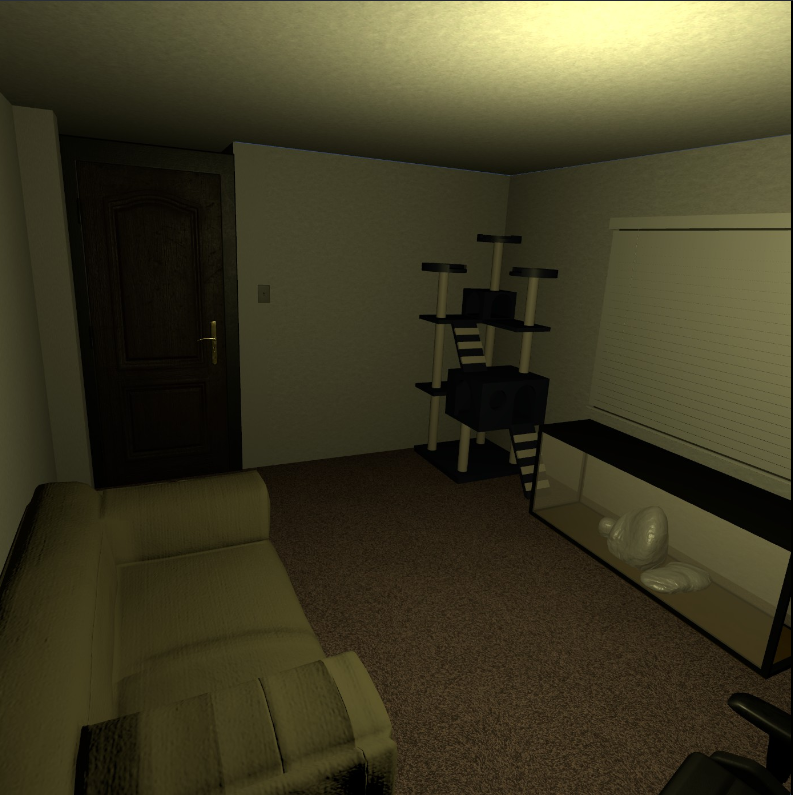
\includegraphics[width=0.25\linewidth]{vrRoom.png}
    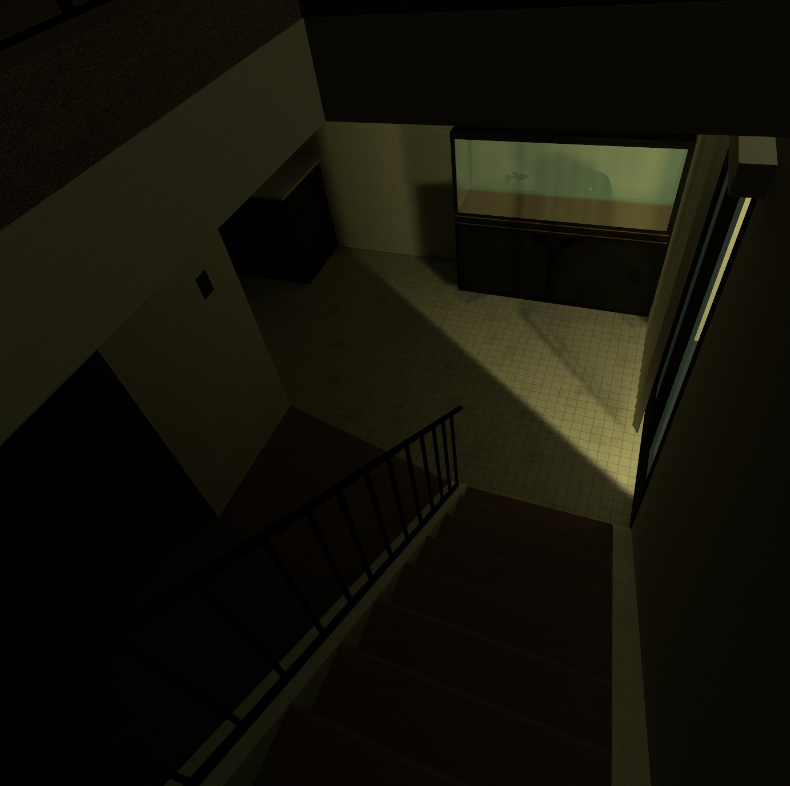
\includegraphics[width=0.25\linewidth]{stairs.png}
    \caption{Examples of sections of the house users traversed in VR}
    \label{fig:2}
\end{figure}
\begin{figure}
    \centering
    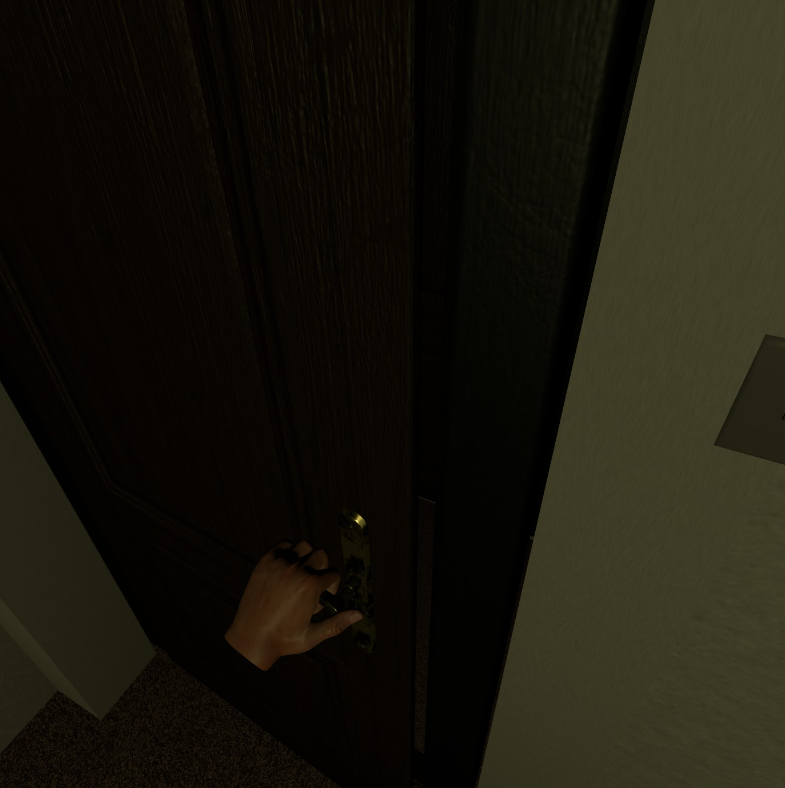
\includegraphics[width=0.25\linewidth]{door.png}
    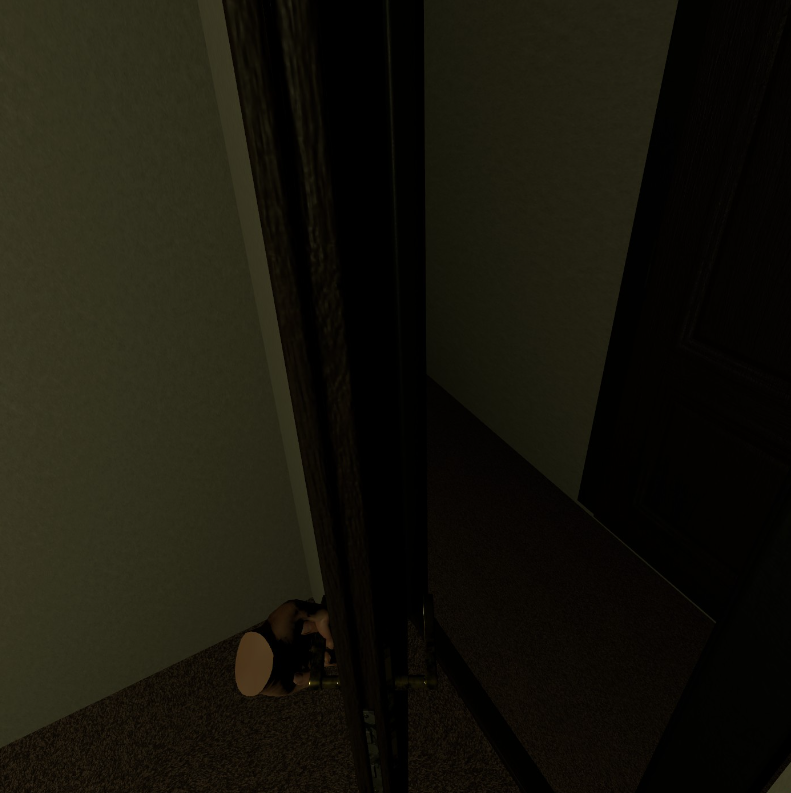
\includegraphics[width=0.25\linewidth]{door2.png}
    \caption{Interactivity implemented through door to keep users engaged.}
    \label{fig:2.1}
\end{figure}
\begin{figure}
    \centering
    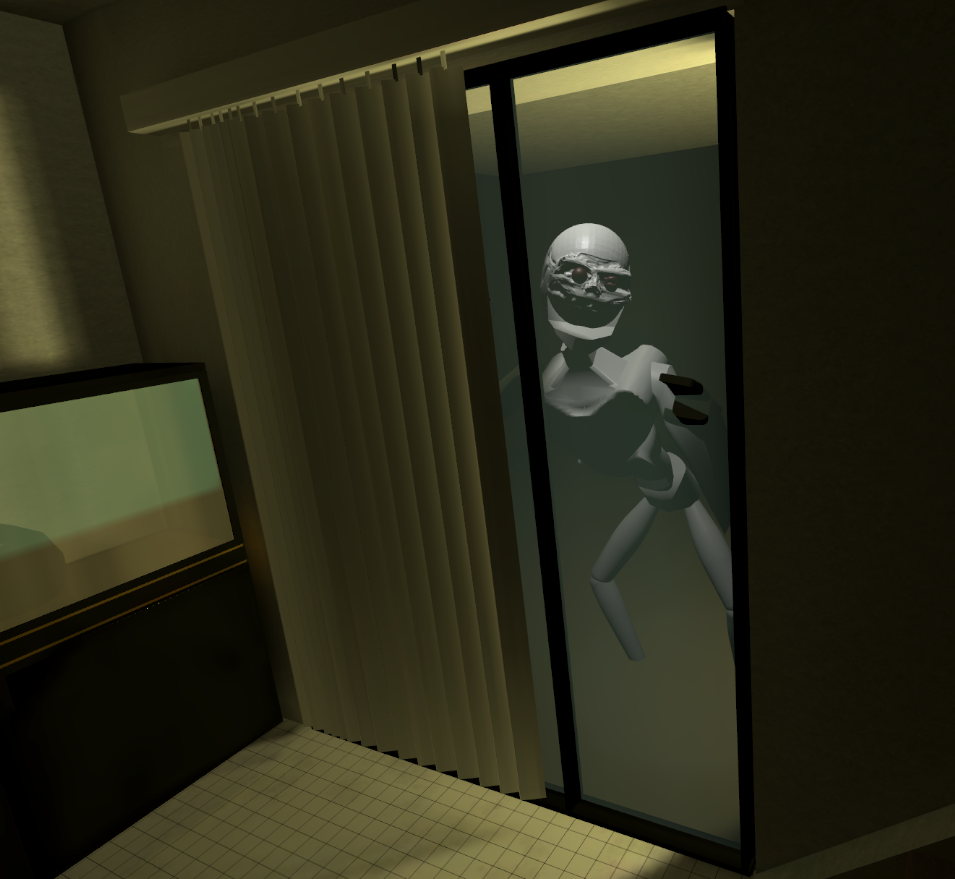
\includegraphics[width=0.5\linewidth]{monster.png}
    \caption{Monster used to jump-scare participants near end of task2}
    \label{fig:2.2}
\end{figure}
The main piece of software used to record heart rate data from participants was a mobile application called \textit{Heart Rate Variability Logger} published by A.S.M.A. B.V, this allowed us to record heart rate data and export it as a csv file to be analyzed. The application was ran on an apple IPhone 14, this helped during sections of the study where participants heart rate was monitored in real time. 
The VR horror game participants played as part of the study was our second piece of software. It was developed in Unity and was modeled one to one on the house where the study took place which can be seen in \autoref{fig:2}. To add the interactivity talked about in \cite{10.1145/3582437.3582482}, the door to leave the tutorial room was designed with physics that the participant could interact it by physical grabbing the handle as seen in \autoref{fig:2.1}. Two methods were used to try and cause fear in participants during the game, sound design with creaking steps and a slamming door while walking away from the tutorial room and a monster suddenly appearing with a sound effect near the bottom of the stairs. This monster can be seen in \autoref{fig:2.2} and was designed with the research of \cite{intel:/content/journals/10.1386/jgvw.2.1.3_1} in mind; being human-like to try and appear uncanny.

\subsection{Procedure}
\begin{figure}
    \centering
    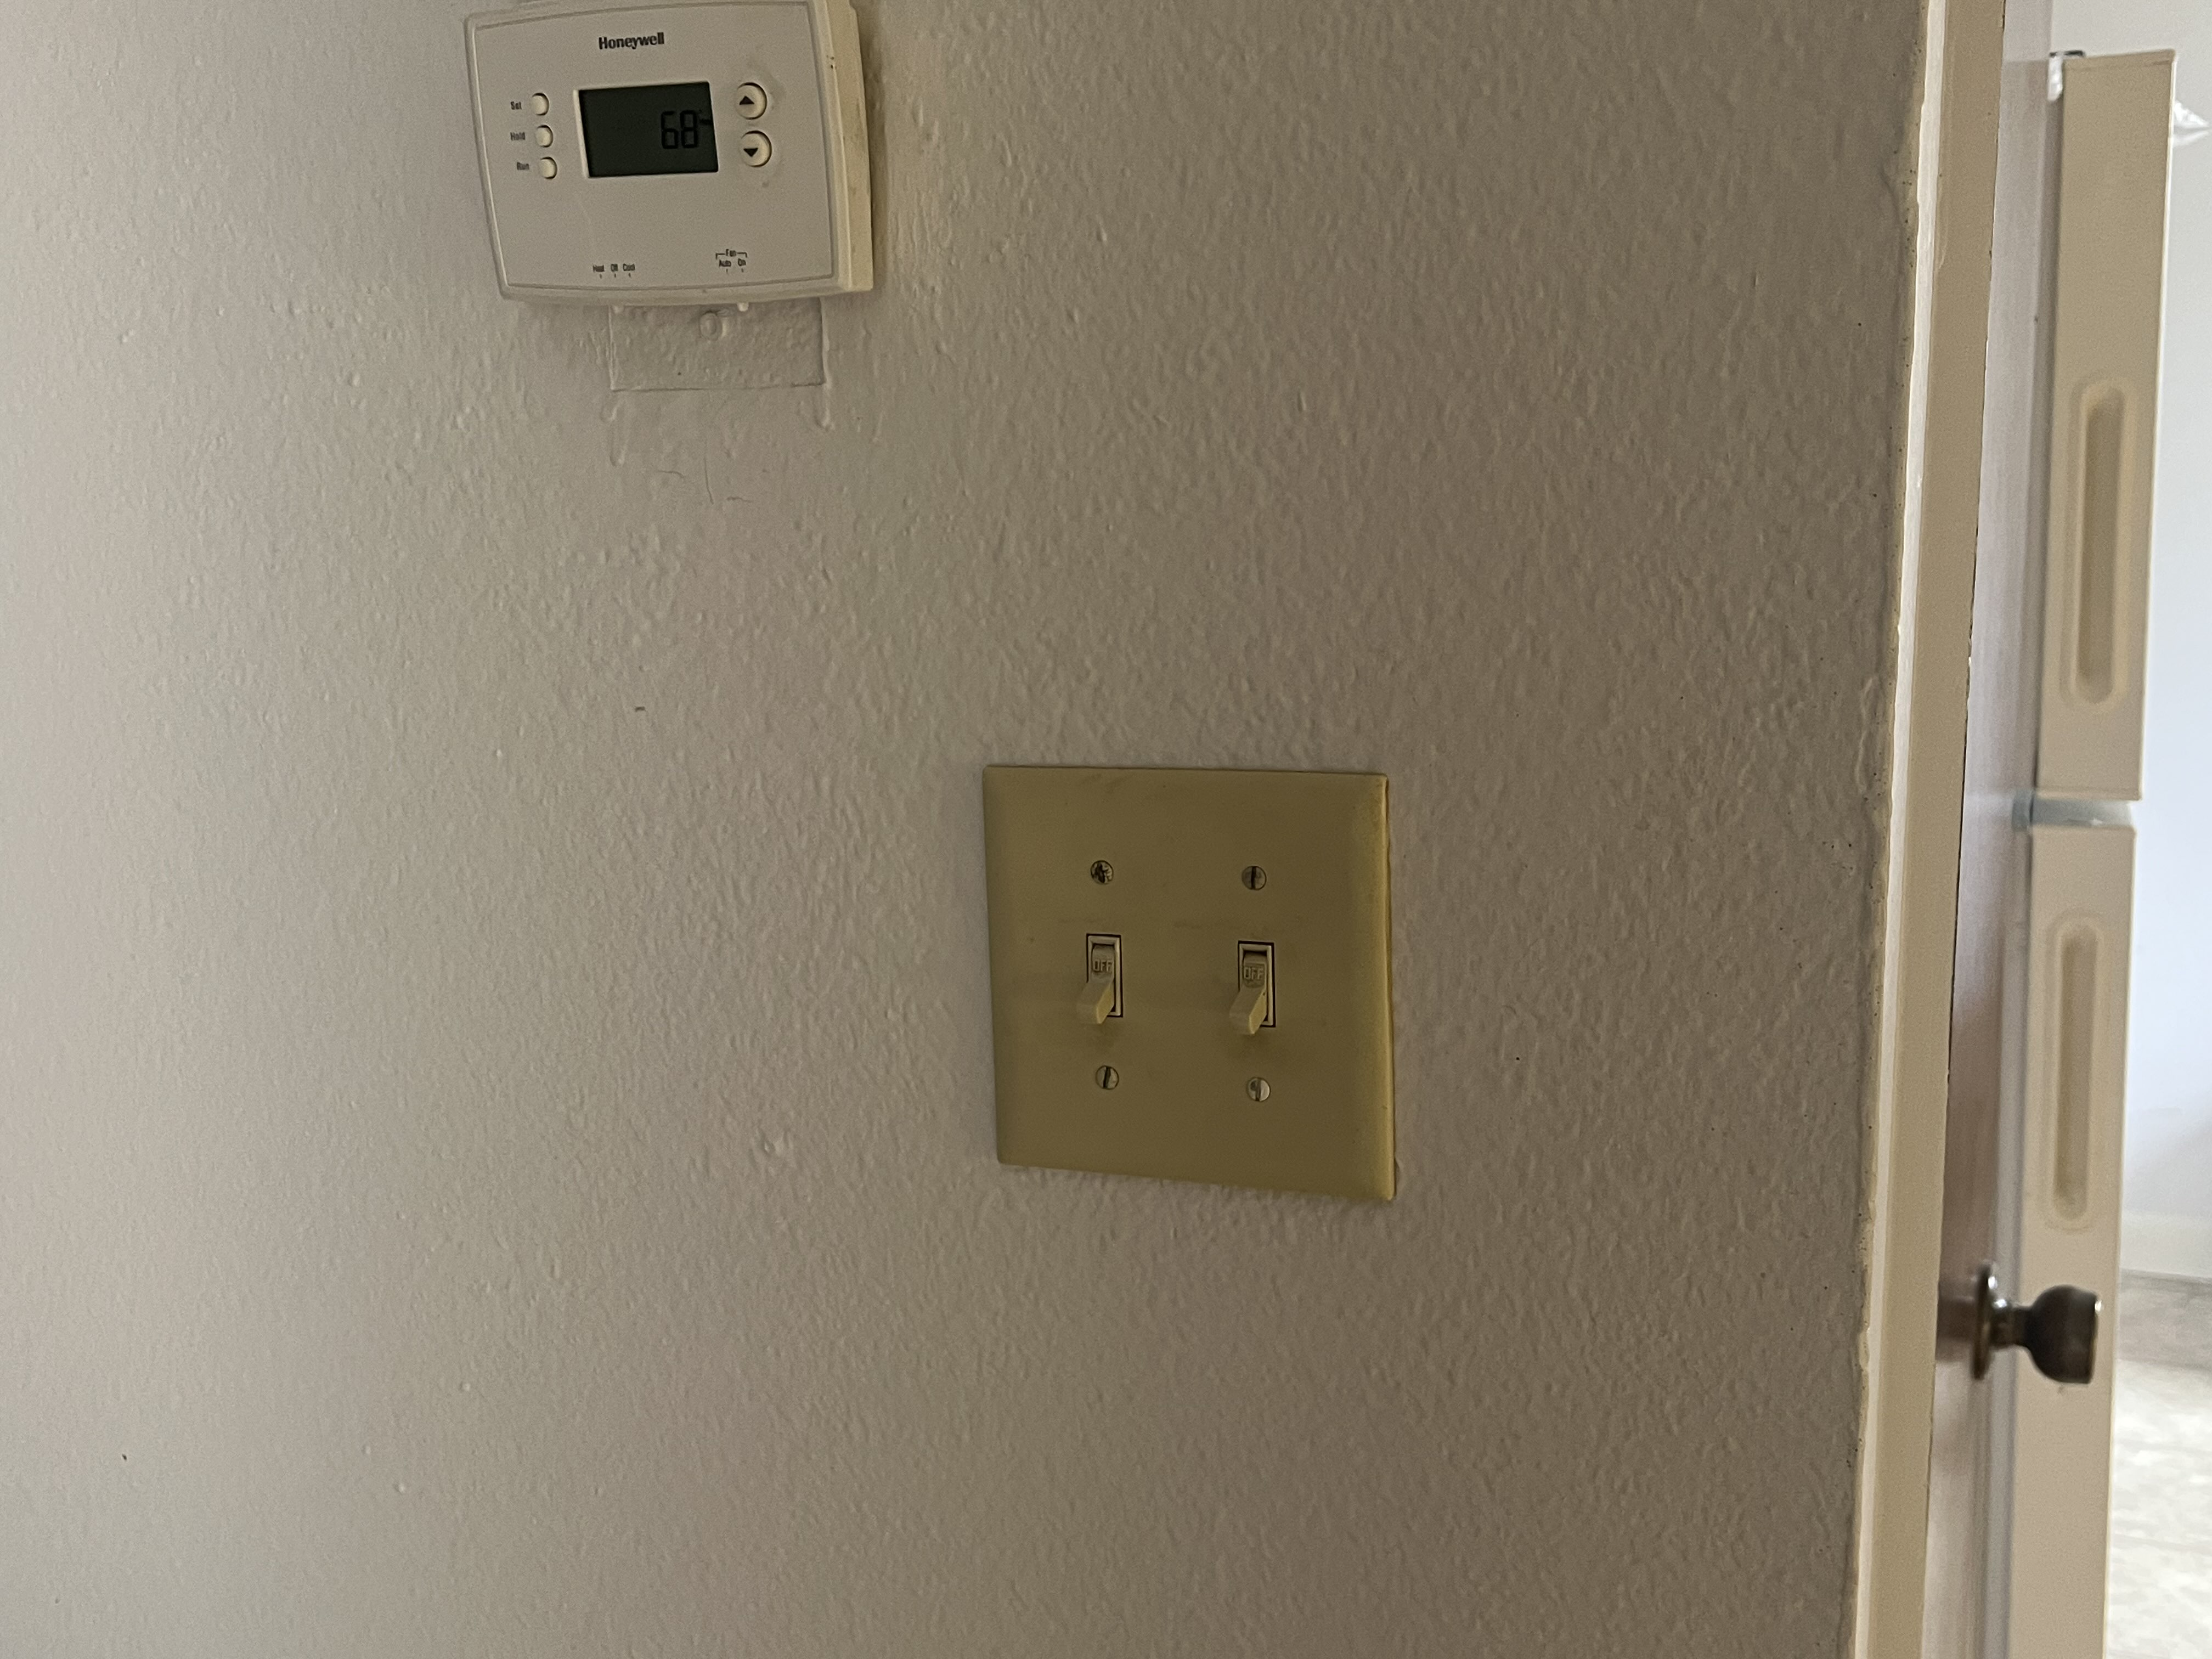
\includegraphics[width=0.25\linewidth]{light-house.jpg}
    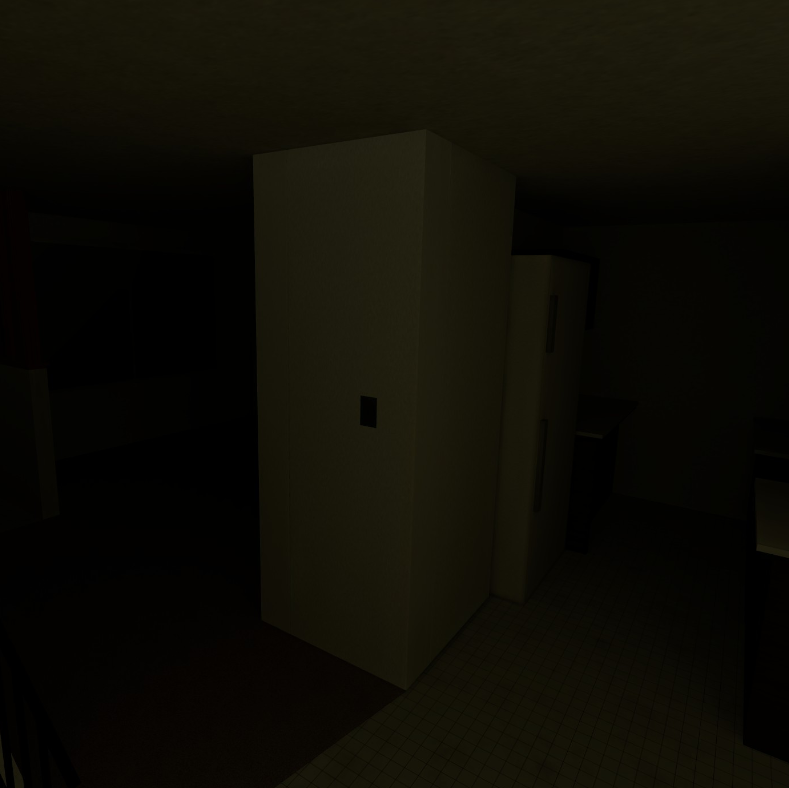
\includegraphics[width=0.25\linewidth]{light-game.png}
    \caption{Left is real-life task, right is VR task.}
    \label{fig:3}
\end{figure}
When participants arrived they given a consent form as well as a verbal explanation of the goal of the study and what they would be asked to do; this was done at the front entrance of the house. Once participants had signed the consent form they were shown a light switch on the wall and told that they would be tasked to flip this light switch three times, twice in real life and once in a VR recreation of the house \autoref{fig:3}. This action was defined to them as the task.

After this participants were taken to a room of the house where the VR equipment and a couch were setup, they were then equipped with the heart rate monitor. At this point they were told to sit on the couch until their heart rate settled, this heart was determined to be a good resting heart rate to let participants to return to after each completion of the task. Once settled participants were told to go complete the task; the time they left and returned to the room was logged in order to find the average heart rate.

After returning participants were asked to sit on the couch again until their heart rate returned to the resting BPM determined before completing the task for the first time. During this period the controls for the VR horror game were explained and demonstrated. Once heart rate settled they were assisted in putting on the VR headset and given a walk through of how to use the controls again. At this point participants were told to complete the task in the VR horror game modeled after the house, start and end time were logged.

Once participants had completed the VR horror game, they were asked to sit on the couch for a final time to allow heart rate to return to resting level. Once heart rate had returned to resting level they were told to complete the task in the real house again; the time they left and returned was logged. After they returned they were told that the study was completed. While completion time of the study varied depending on how long heart rate took to return to resting level, time to complete tasks, and time to complete horror game; most participants completed everything in 10-15 minutes.

\subsection{Design}

The experiment was a single factor with two levels within-subject design. The independent variable in this was if participants had been exposed to the VR horror game or not, a before and after measurement. The dependent variable was participant heart rate averaged over the completion of the task before and after playing the VR horror game. An issue that we ran into with this design was the issue of noise in the data, since heart rate can vary by person and can be influenced by so many things outside of the control of the study there could be any number of things impacting that we would have no clue about. The total number of trials was 24 (=12 participants X 2 measurements).

\section{Results and Discussion}
\begin{table}
    \centering
    \begin{tabular}{cccc}
    \toprule
        & T1 & T2 & T3 \\
        \midrule
        P1 & 73.9 & 103.9 & 80.1 \\
        P2 & 95.1 & 108.7 & 102.7 \\
        P3 & 103.8 & 90.5 & 90.8 \\
        P4 & 106.5 & 111.8 & 108.3 \\
        P5 & 91.9 & 83.1 & 73.5 \\
        P6 & 87.6 & 99.4 & 88.5 \\
        P7 & 77.1 & 94.1 & 78.8 \\
        P8 & 81.9 & 89.1 & 85.2 \\
        P9 & 71.8 & 65.9 & 73.3 \\
        P10 & 87.3 & 74.7 & 68.6 \\
        P11 & 118.4 & 93.6 & 102.2 \\
        P12 & 80.9 & 75 & 85.4 \\
        \bottomrule
    \end{tabular}
    \caption{Average heart rate over each trial.}
    \label{tab:averages}
\end{table}

\begin{table}[ht]
    \centering
    \begin{tabular}{|c|c|c|c|c|c|}
    \hline
    Effect        & df & SS       & MS       & F    & p      \\ \hline
    Participant   & 11 & 3424.043 & 311.277  &      &        \\ \hline
    F1            & 1  & 62.727   & 62.727   & 1.220 & 0.2929 \\ \hline
    F1 x Par      & 11 & 565.383  & 51.398   &      &        \\ \hline
    \end{tabular}
    \caption{ANOVA Table of all participants}
    \label{tab:anovaAll}
\end{table}

\begin{table}[ht]
    \centering
    \begin{tabular}{|c|c|c|c|c|c|}
    \hline
    Effect        & df & SS       & MS       & F    & p      \\ \hline
    Participant   & 5 & 1466.114 & 293.223  &      &        \\ \hline
    F1            & 1  & 38.521   & 38.521   & 10.414 & 0.0233 \\ \hline
    F1 x Par      & 5 & 18.494  & 3.699   &      &        \\ \hline
    \end{tabular}
    \caption{ANOVA Table of participants afraid of game}
    \label{tab:anovaAfraid}
\end{table}

\begin{table}[ht]
    \centering
    \begin{tabular}{|c|c|c|c|c|c|}
    \hline
    Effect        & df & SS       & MS       & F    & p      \\ \hline
    Participant   & 5 & 1944.728 & 388.946  &      &        \\ \hline
    F1            & 1  & 303.008   & 303.008   & 5.651 & 0.0634 \\ \hline
    F1 x Par      & 5 & 268.087  & 53.617   &      &        \\ \hline
    \end{tabular}
    \caption{ANOVA Table of participants not afraid of game}
    \label{tab:anovaNotAfraid}
\end{table}
Heart rate data during each task was averaged for each task and can be seen in \autoref{tab:averages}. Data for task 2, while not useful for the goal of the experiment since it's the average heart rate while playing the game, still allows us to see which participants felt fear during the game and which didn't. This proved a useful identifier when performing ANOVA on the data; for all participants \(p=0.2929\) which can be seen in \autoref{tab:anovaAll}, this is greater than 0.05 the horror game did not have a statistically significant impact on the heart rate during the task before and after.

The average heart rate for T2, when participants were playing the horror game, in \autoref{tab:averages} allows us to split the data into people who showed fear in the game (referred to after this as group1) and those who did not (referred to after this as group2); this decision was made base on if heart rate was higher than T1 heart rate. Participants P3, P5, P9, P10, P11, and P12 were deemed to not have shown fear in the game. ANOVA was performed again on each of these subgroups, those who displayed fear can be seen \autoref{tab:anovaAfraid} while those who didn't can be seen in \autoref{tab:anovaNotAfraid}. The VR horror game once again did not have a statistically significant impact on group2 with a \(p=0.0634\). This changed for group1 with a \(p=0.0233\) which was below the threshold of \(0.05\) to be significant.

We believe a possible explanation for why the VR horror game was only statistically significant for group2 is because group1 was never afraid in the first place. This could be due to the game used in the experiment not utilizing techniques that would elicit a response from them, having a higher tolerance for fear in general, or not being as engaged by the experiment in general. There is also a possibility that since not every participant showed fear to the game, we don't have large enough sample of either group. What we did find though was that when people do show fear in VR horror it does seem to elicit a change in response to their environment afterwards.

\section{Conclusion}
Overall, we found that when people have a high heart rate while playing a VR horror game it is reflected in a high heart rate while replicating a similar task even after given time to return back to a resting heart rate. If someone's heart rate isn't effected by a VR horror game then their heart rate does not show statistically significant change when completing a similiar task afterwards. 

Given additional time there are several things we would change; the big change would be getting a larger sample size of both groups of people. Though it is hard to tell before playing who will show fear in the heart rate, we would try to focus more on building a better game in order to limit the amount of people who don't show a response to it. Some of the several ideas we had were to increase the length or to add more interaction, all of the main elements to cause fear where static such as audio cues and a jump scare and dynamic elements might cause a response in more participants which would give more data to support or disprove \autoref{tab:anovaAfraid}.

%%
%% The next two lines define the bibliography style to be used, and
%% the bibliography file.
\bibliographystyle{ACM-Reference-Format}
\bibliography{sample-base}
\end{document}
\endinput
%%
%% End of file `main.tex'.
